% !TeX root = Poster/tikzposter.tex
\documentclass[25pt,a0paper,portrait]{tikzposter}
\usepackage[utf8]{inputenc}
\usepackage[table]{xcolor}
\usepackage{graphicx}
\usepackage{amsmath}

% Allow compilation both from repo root (Poster/images/...) and from within
% the Poster/ directory (./images/...).
\graphicspath{{./images/}{Poster/images/}}

\setlength{\columnsep}{0.8cm}

\title{CPI Forecasting in Germany Using ARIMA, ETS, and SARIMA}
\author{Siddhanth Sharma, Nayan Chavan, Gargi Barve}
\titlegraphic{%
	
\includegraphics[height=4.0cm]{logo_hs_technik}
	\hfill
	
\includegraphics[height=4.2cm]{logo}%
}

\usetheme{Desert}

\begin{document}

\maketitle

\begin{columns}

\column{0.5}
{
	\colorlet{blocktitlebgcolor}{blue}
	\block{Problem Description}
	{
		Germany's Consumer Price Index (CPI) is a central indicator of inflation, cost-of-living change, and purchasing power. Because it is published regularly and closely monitored by policy makers, researchers, and businesses, forecasting its future path is a meaningful time-series task. This project predicts future German CPI values using only historical monthly CPI observations and no external explanatory variables.

		The data comes from the official Destatis GENESIS database, table 61111-0002, and is modeled as a \textbf{univariate economic time series}. Each observation contains a monthly timestamp and the CPI index level, with base year \textbf{2020 = 100}. By excluding external predictors, the study isolates the forecasting information contained in the CPI series itself.

		The goal is not only to generate forecasts, but also to determine which classical forecasting approach is most suitable for this type of macroeconomic data. Three established model families are compared: \textbf{ARIMA}, \textbf{ETS}, and \textbf{SARIMA}. Evaluation is based on a chronological holdout design that reflects a realistic forecasting setting.

		\vspace{0.8em}
	}

	\block{Data \& Split}
	{
		\begin{itemize}
			\item \textbf{Raw series:} 422 monthly observations from \textbf{January 1991 to February 2026}.

			\item \textbf{Training set:} \textbf{January 1991 to February 2024}.

			\item \textbf{Test set:} \textbf{March 2024 to February 2026}.

			\item \textbf{Forecast horizon:} \textbf{24 months ahead}.

			\item Although training starts in 1991, the chart below shows a zoomed view from \textbf{2020} for readability.
		\end{itemize}
	}

	\block{Challenges}
	{
		The main project challenges came from both the statistical behavior of CPI and the methodological requirements of a fair model comparison:

		\begin{itemize}
			\item \textbf{Long-term upward trend:} CPI is a price-level index and therefore tends to rise over long periods when inflation is positive. This creates a non-stationary structure that requires explicit trend handling or differencing.

			\item \textbf{Monthly temporal dependence:} Consecutive CPI values are strongly related, so the models must capture autocorrelation and persistence across months.

			\item \textbf{Possible yearly seasonality:} Because the data is observed monthly, repeating annual patterns may exist. The comparison therefore needs methods that can explicitly represent a seasonal cycle of length 12.

			\item \textbf{Recent inflation changes:} The later part of the series contains the strong inflation movement after 2021, making forecasting more demanding than in a more stable period.

			\item \textbf{Model comparability:} Forecasts can only be compared meaningfully if they use the same training window, forecast horizon, and evaluation metrics. Random splits would introduce leakage, so a chronological holdout was necessary.
		\end{itemize}

		\vspace{0.6em}
	}

	\block{Train, Test \& Forecasts}
	{
		\vspace{0.5em}
	    \begin{center}
			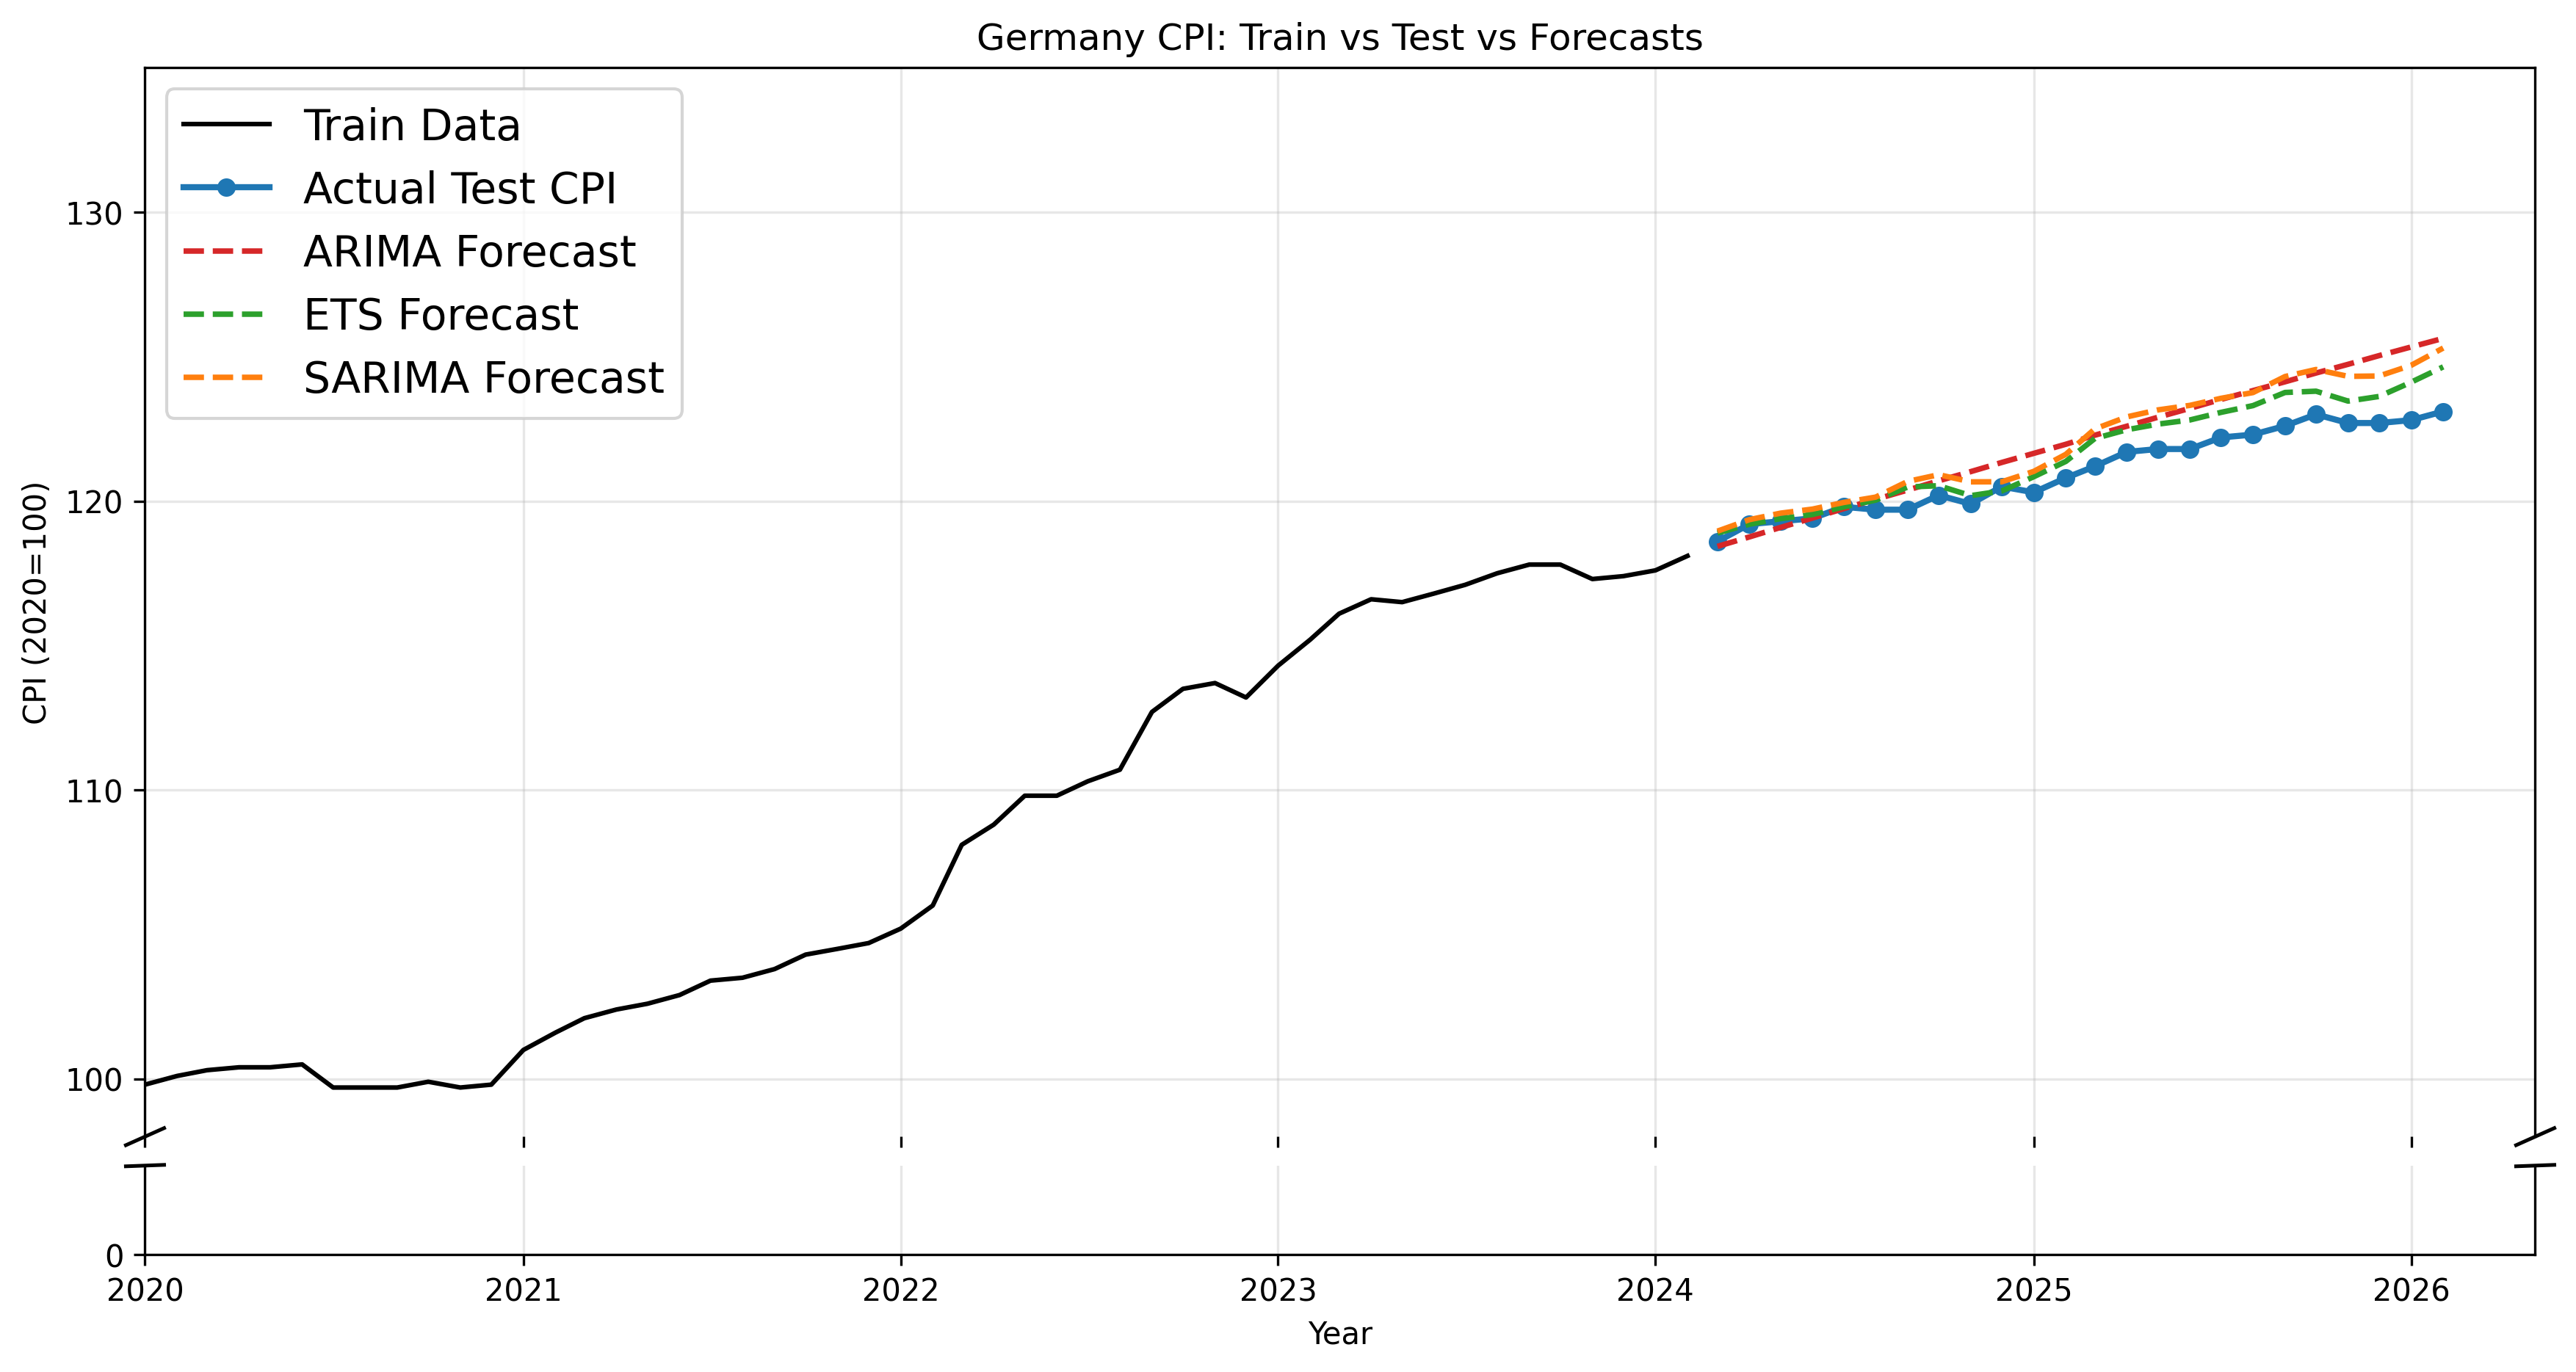
\includegraphics[width=\linewidth]{forecast_comparison}
		\end{center}
		\vspace{0.5em}
	}
}

\column{0.5}
{
	\colorlet{blocktitlebgcolor}{blue}
	\block{Forecast Comparison}
	{
		\begin{center}
			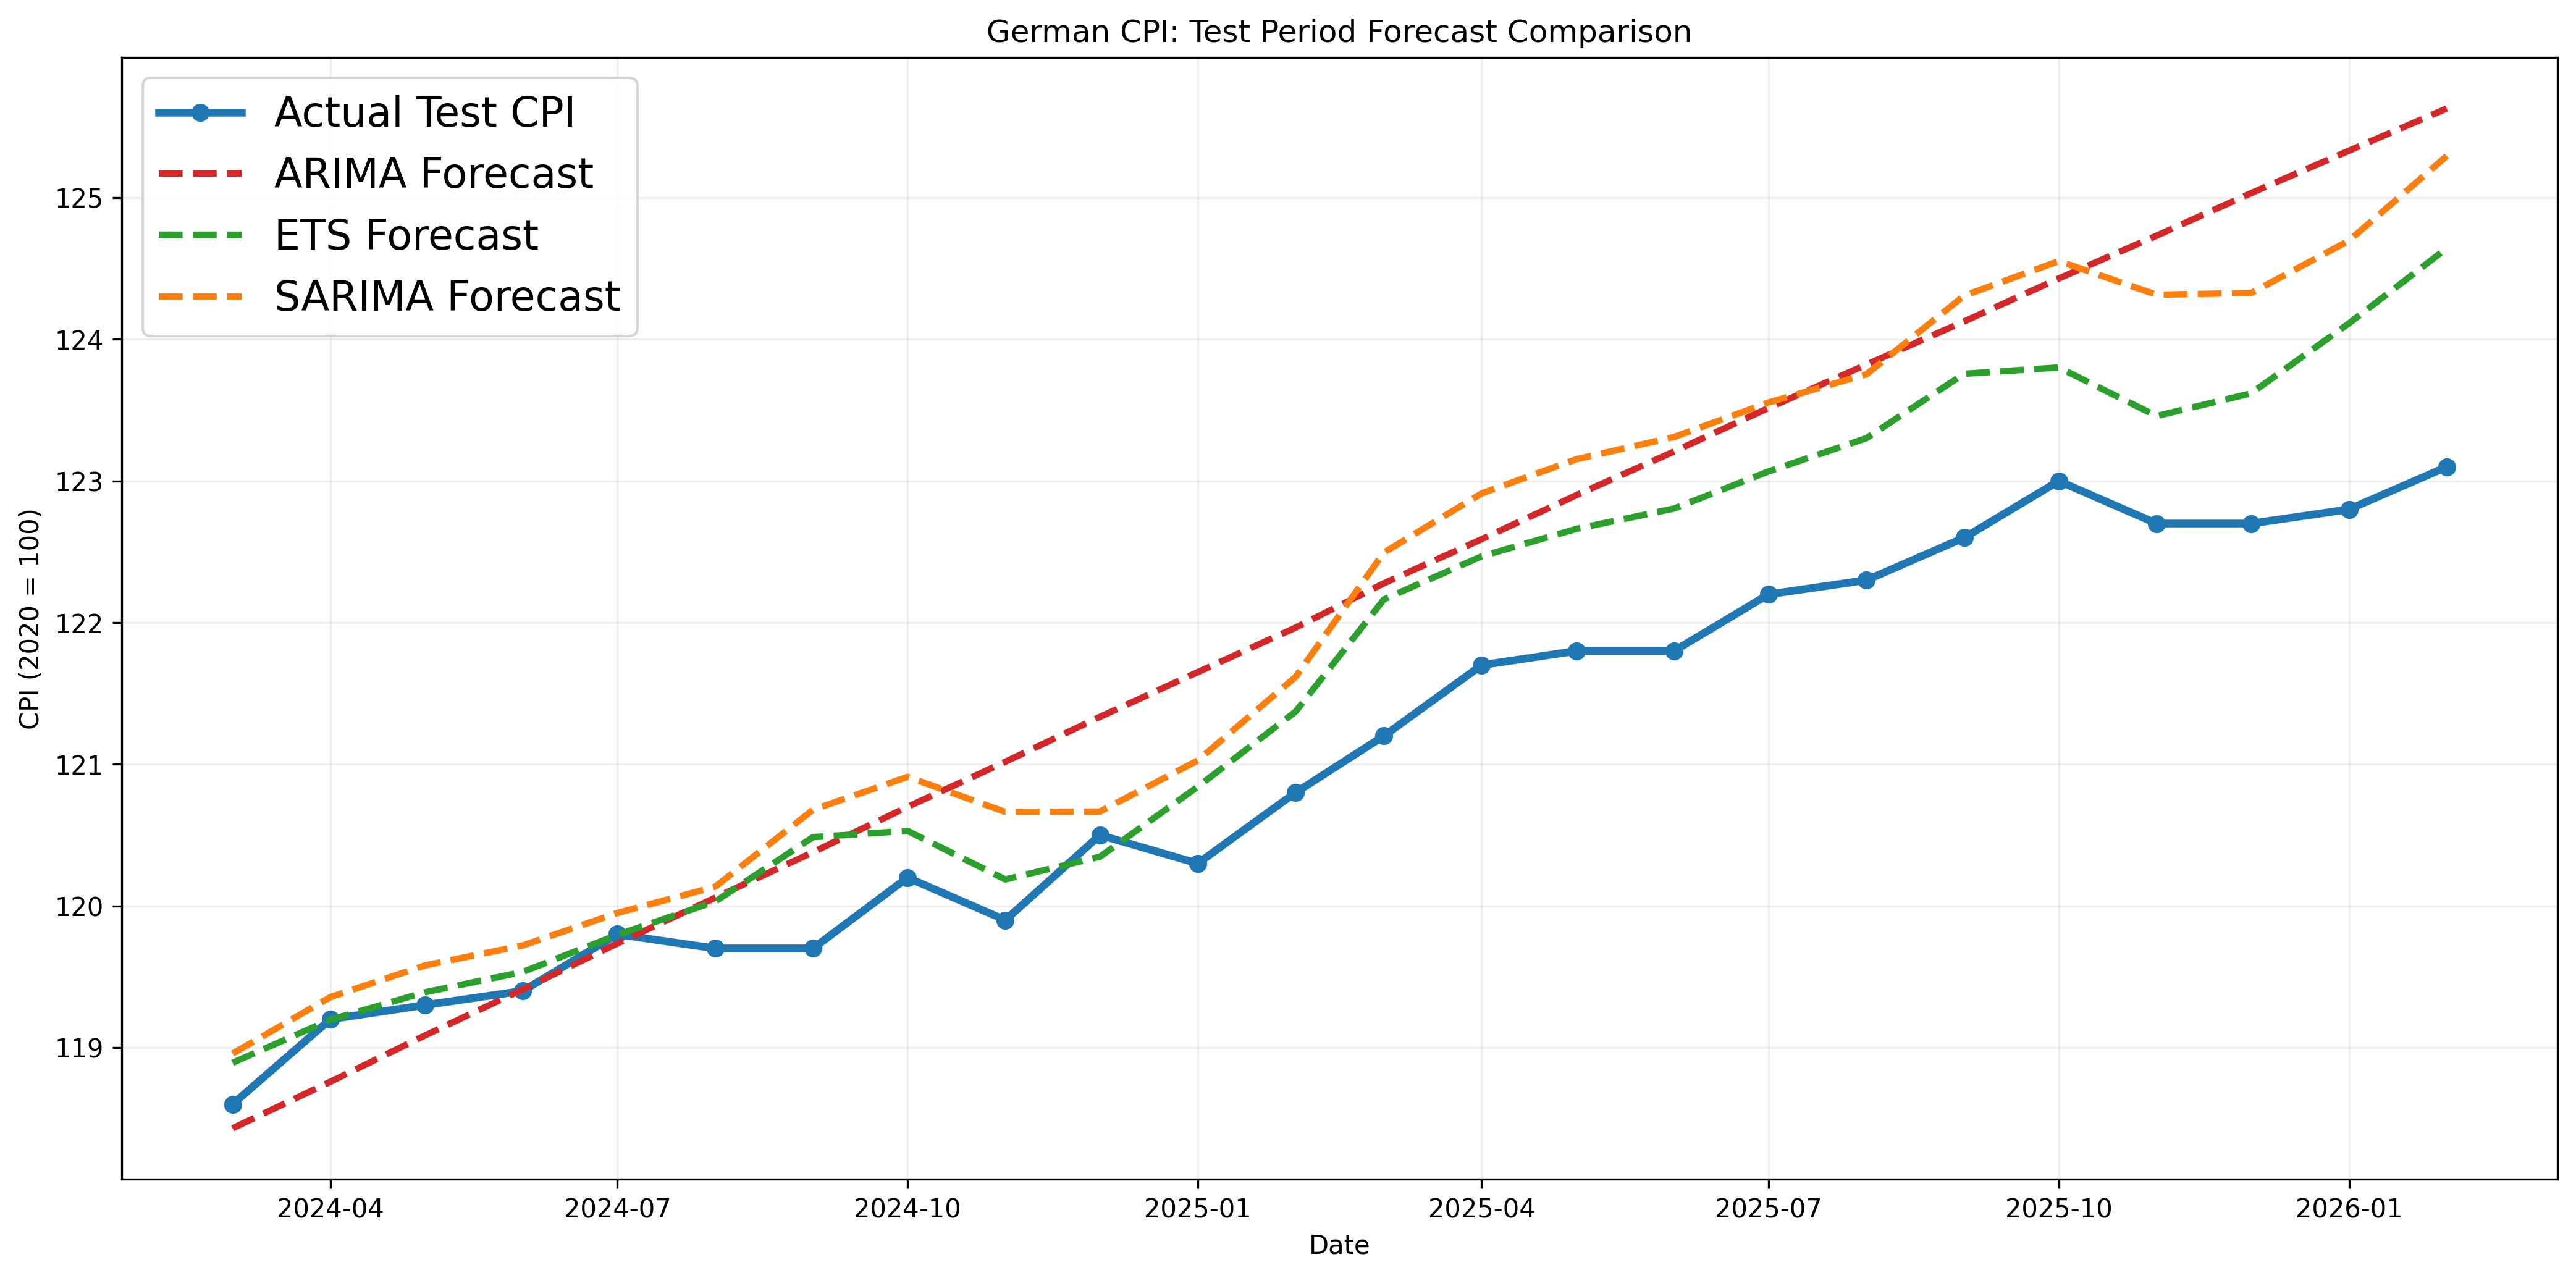
\includegraphics[width=\linewidth]{test_forecast_comparison}
		\end{center}
	}

	\block{Solutions}
	{
		The project addressed these challenges through model selection and evaluation:

		\begin{itemize}
			\item \textbf{Handling the upward trend:} ARIMA and SARIMA use integrated components, so differencing reduces non-stationarity before the remaining structure is modeled. ETS addresses the same issue differently by modeling level and trend directly through additive error-trend-seasonal components.

			\item \textbf{Modeling temporal dependence:} ARIMA(1,1,1) was selected as a compact non-seasonal baseline. It tests whether short-term autoregressive and moving-average behavior alone is sufficient to describe CPI dynamics.

			\item \textbf{Representing seasonality:} SARIMA(1,1,1)(1,1,1)$_{12}$ extends ARIMA with seasonal terms and a seasonal period of 12, matching the monthly structure of the data. ETS(A,A,A) was also included because it can represent additive level, additive trend, and additive seasonality directly and interpretably.

			\item \textbf{Avoiding leakage:} The final 24 months were kept unseen during training. All three models were fitted on the same historical window and used to forecast the same future horizon, making the reported errors directly comparable.

			\item \textbf{Interpretable comparison:} Performance was reported using RMSE, MAE, and MAPE. Together, these metrics show absolute CPI index error as well as relative percentage error, giving a balanced view of forecast quality rather than relying on a single measure.
		\end{itemize}

		\vspace{0.6em}
	}

	\block{Results}
	{
		\vspace{-5pt}
		\begin{center}
		\renewcommand{\arraystretch}{1.18}
		\setlength{\tabcolsep}{60pt}
		\begin{tabular}{|c|c|c|c|}
			\hline
			\textbf{Model} & \textbf{RMSE} & \textbf{MAE} & \textbf{MAPE} \\
			\hline
			ARIMA(1,1,1) & 1.3262 & 1.1086 & 0.9099\% \\
			\textbf{ETS(A,A,A)} & \textbf{0.7697} & \textbf{0.6453} & \textbf{0.5298\%} \\
			SARIMA(1,1,1)(1,1,1)$_{12}$ & 1.1909 & 1.0268 & 0.8431\% \\
			\hline
		\end{tabular}
		\end{center}

		\vspace{1em}

		\begin{itemize}
			\item \textbf{Key takeaway:} ETS(A,A,A) produced the most accurate forecasts for German monthly CPI over the 24-month test horizon.

			\item \textbf{Best overall model:} ETS(A,A,A) achieved the lowest RMSE, MAE, and MAPE, so the conclusion remains stable across all error measures.

			\item \textbf{Forecast accuracy:} Its MAE of \textbf{0.6453} means the forecast was, on average, less than one CPI index point away from the observed value. Its MAPE of \textbf{0.5298\%} shows that the relative error remained very small over the test period.

			\item \textbf{Relative improvement:} ETS reduced RMSE by about \textbf{42\%} versus ARIMA and \textbf{35\%} versus SARIMA, showing a meaningful practical gain.

			\item \textbf{Interpretation:} The result indicates that additive level, trend, and seasonal components describe the CPI series particularly well in the evaluation period. In contrast, the non-seasonal ARIMA model was less able to capture recurring monthly structure, while SARIMA improved on that limitation but still remained behind ETS.

			\item \textbf{Future work:} A next step would be to include external drivers such as energy prices, wages, or interest rates and test whether multivariate models improve forecast accuracy further. This would help determine whether the remaining forecast error comes mainly from internal time-series structure or from outside economic shocks.
		\end{itemize}

		\vspace{0.4em}
	}
}

\end{columns}

\end{document}
